\documentclass[11pt,a4paper]{scrartcl}

\usepackage[ngerman,english]{babel}
\usepackage{graphicx}
\graphicspath{{pics/}}

\title{Hair Simulation with OpenCL}
\author{Etienne Gramlich \& Heiko Ettwein}


\begin{document}
\maketitle
\tableofcontents
\newpage
\pagenumbering{arabic}

\section{Introduction}

\subsection{Project Description}


\section{Implementation}

\subsection{Architecture}

\subsection{OpenCL}

\subsection{OpenGL}


\section{Hair Physics}
simple force model, no bounding boxes, small random differences of hair masses

\subsection{Force Model}
acceleration vectors, velocity, mass, linear combination of vectors

\subsubsection{Gravity}
gravitational force

\subsubsection{Elasticity}
link force \\ spring force

\begin{figure}[htbp]
\centering
\fbox{
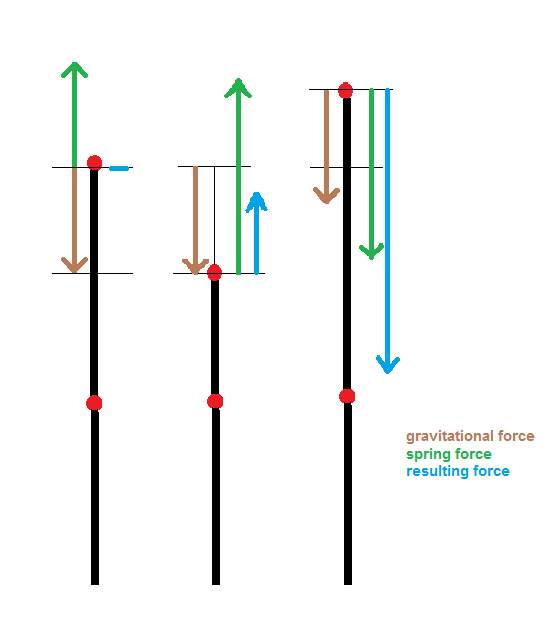
\includegraphics[width=1.0\textwidth]{SpringForce.png}
}
\caption{Spring force}
\end{figure}

\begin{figure}[htbp]
\centering
\fbox{
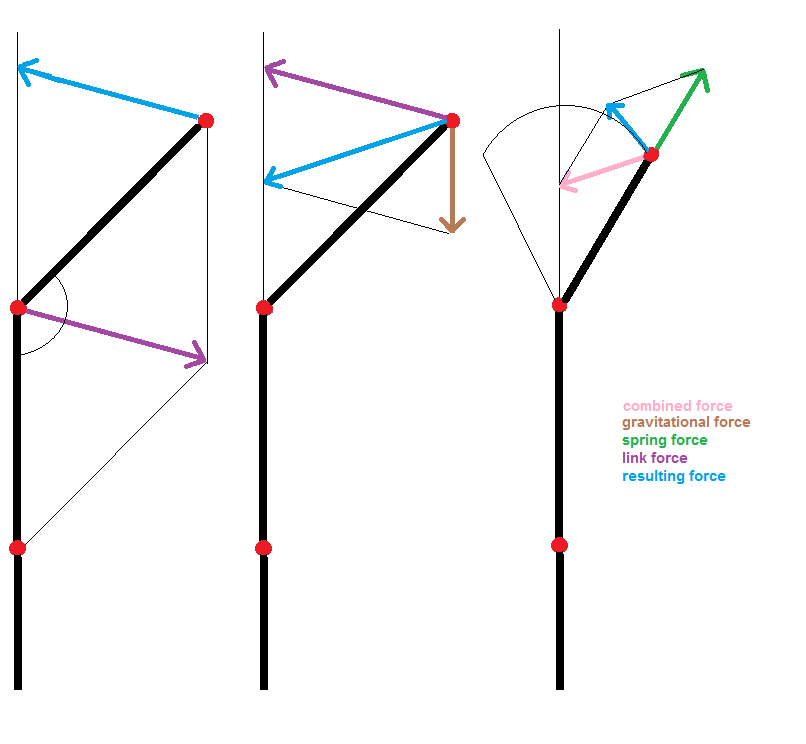
\includegraphics[width=1.0\textwidth]{CombinedForce.png}
}
\caption{Combination of all forces}
\end{figure}


\newpage
\subsubsection{Wind}
wind force \\ control direction and intensity (maximum force and interval)


\section{Conclusion}


\end{document}